% !TEX root = sum1.tex
\section{Problem Description}
In this section, we consider the dynamic seat assignment problem with social distance.

% give the description of the seat planning problem with social distance.

% dynamic seat assignment problem, which is suitable for commercial use in cinemas and concerts.

\subsection{Dynamic Seat Assignment Problem with Social Distance}\label{dynamic_demand}

Generally speaking, there are two ways to purchase tickets for concerts or movies: no seat selection when booking and seat selection when booking. We consider the following dynamic demand situations, seat assignment after booking period and seat assignment when booking.

For reservations without seat selection, the seat assignment will not be made immediately. Instead, the decision-maker must either accept or reject each request during the making-reservation stage. After the reservation deadline, the seller will inform the customers of the seat layout information before admission. For example, in singing concert venues with many seats and high ticket demand, organizers usually do not determine the seats when booking and then inform customers of the seat information after the overall seat layout is determined.

In contrast, for seat assignment when booking, the specific procedure will be changed to meet the requirements of social distancing. The seat assignment will be arranged before groups book their tickets, and the groups will only need to choose seats of the corresponding size when booking. For example, in movie theaters or small concerts with relatively few seats, the attendance rate is usually low enough to allow free selection of seats directly online. Early seat planning can satisfy the requirement of social distancing and save costs without changing seat allocation. The seat assignment could remain for one day because the same film genre will attract the same feature of different group types.

Our study mainly focuses on the latter situation where customers come dynamically, and the seat assignment needs to be made immediately without knowing the number and composition of future customers. In Section 6, we also consider the situation where the seat assignment can be made after the booking period.


Consider a set of groups, each consisting of no more than $m$ people, to be assigned to a set of seats. These groups are denoted by a demand vector, $\mathbf{d} = (d_1, \ldots, d_m)$. Each element, $d_i, 1 \leq i \leq m$, indicates the number of group type $i$ containing $i$ people. For illustration, we consider the layout as $N$ rows, each row with $S_{j}$ seats, $j = 1, \ldots, N$. 


We use a vector $\mathbf{S}= (S^{r}_1, S^{r}_2, \ldots, S^{r}_{N})$ to record the remaining capacity of rows, in every period the group can decide which row to sit. Let $V_{t}(\mathbf{S})$ denote the maximal expected value to go at period $t$ with capacity of rows. Let $\mathbf{w} = (s_1+1, \ldots, s_m+1)$ be the number of seats occupied by each group type. There are $T$ periods and the arrival probability of the group type $i$ in each period is $p_i$. 

The dynamic programming formulation for this problem is
$$V_{t}(\mathbf{S}) = \sum_{i \in m} p_i \max\{ {[V_{t-1}(\mathbf{S}- \mathbf{w} \circ \mathbf{e}_{i})+ s_i]}, {V_{t-1}(\mathbf{S})}\}, \mathbf{S} \geq \mathbf{0}, V_{T+1}(\mathbf{S}) = 0,$$

where $\mathbf{e}_{i}$ is the unit vector whose i-th element is 1. $\circ$ is the element-wise product. Initially, we have $\mathbf{S}_{T} = (S_1, S_2, \ldots, S_{N})$. 

As we can see, this dynamic programming falls into the curse of dimensionality due to many seating plan combinations. Even worse, DP only records the remaining seats of each row, cannot reach the goal of assigning to seats at each period. To avoid this complexity, we develop an approach that aims directly at the final seating plans, then make the policy to assign groups. 


% As stated above, we can obtain such a seating plan from stochastic programming. However, it only gives the initial seat assignment without handling the dynamic situation. 


\subsection{Seat Planning with Social Distance}
% In this section we present the model that generates seat assignment under deterministic demands.

% Let the $i-$th group type contain $i$ people. 
% $(d_1, d_2, d_3, d_4) = (3,5,7,6)$

% But our model and formulation allow for a more general layout of the seats. 
In accordance with epidemic prevention requirements, customers from the same group are allowed to sit together, while different groups must maintain social distancing. Specifically, each group must leave one seat empty to maintain social distancing from adjacent groups. Additionally, different rows do not affect each other, meaning that a person from one group can sit directly behind a person from another group.

To achieve the social distancing requirements in the seat planning process, we add one to the original size of each group to create the new size of the group. We also add one dummy seat to each row. Let $s_i = i + 1$ denote the new size of group type $i$, and let $L_j = S_j + 1$ denote the length of row $j$, where $S_j$ represents the number of seats in row $j$.


Then we can illustrate the seat planning for one row below. 

\begin{figure}[ht]
    \centering
    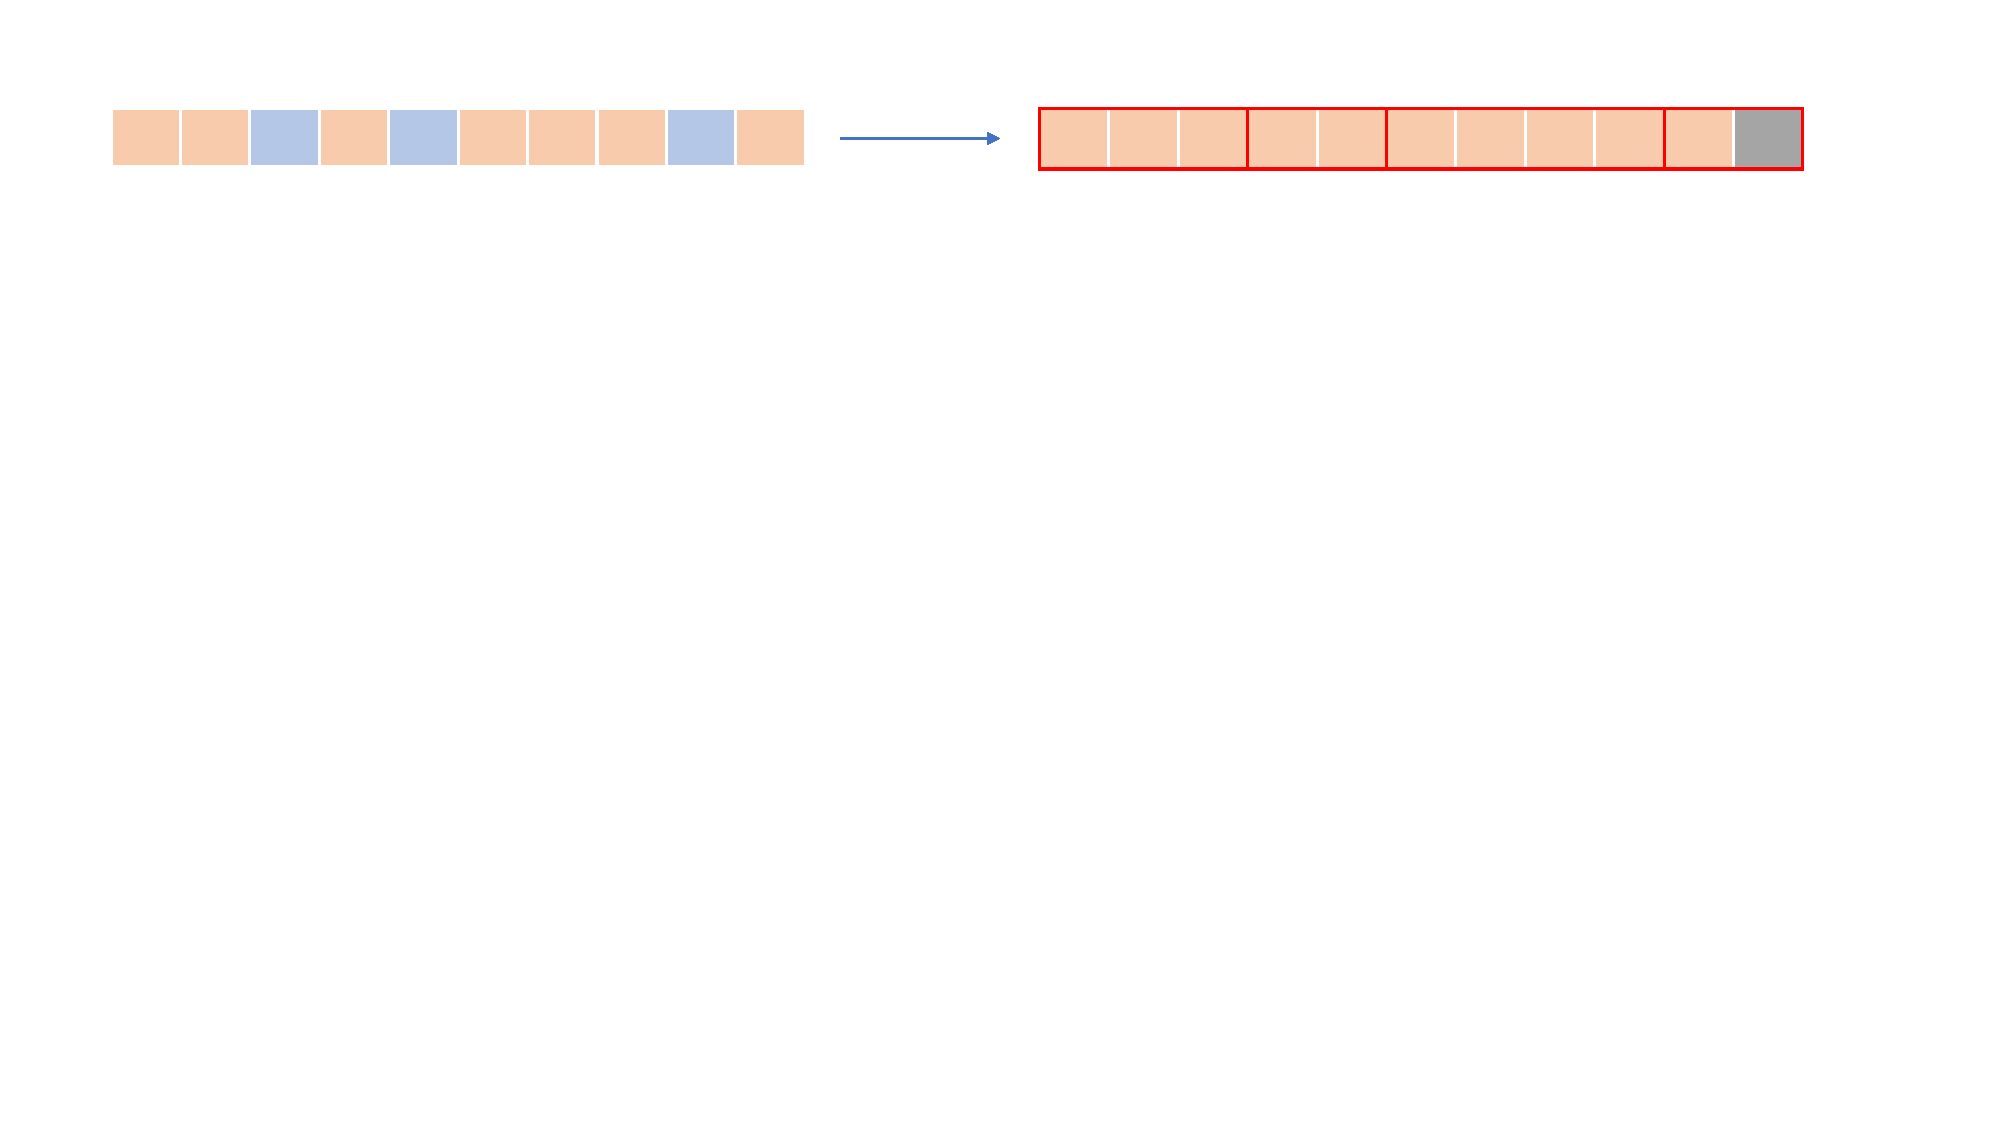
\includegraphics[width = 0.8\textwidth]{./Figures/dummy_seat.pdf}
    \caption{Problem Conversion}
\end{figure}


On the left side of the diagram, the blue squares represent the empty seats required for social distancing, while the orange squares represent the seats occupied by groups. On the right side, we have added one dummy seat at the end of each row. The orange squares surrounded by the red line represent the seats taken by groups in this row, which includes two groups of 1, one group of 2, and one group of 3.

By incorporating these additional seats and designating certain seats for social distancing, we can integrate social distancing measures into the seat planning problem.

To obtain the final seat planning firstly, we develop the scenario-based stochastic programming.
% The number of all seats in each row is called the length of the row.

% when the capacity allows accepting the groups from large to small as many as possible will give an optimal solution.


% Why is it easy to solve this IP?

% If the ratio is the same for the groups, IP will use more branches to obtain an optimal solution.

% $[24,28,8,9]$ 10 rows.
% Total loss: 60; loss of the largest pattern: 5.


% Specifically, we define the concept of target seating plans deemed satisfactory. In making the dynamic seating plan, we will try to maintain the possibility of achieving one of the target seating plans as much as possible.
